\begin{appendices}
  \chapter{Mathematical Appendix}
  \section{Mathematical Notation}
  \label{app:math_notation}

  This section provides a reference for the mathematical notation used throughout this thesis. \ai{Mathematical formulas used here have been generated by AI.}

  \begingroup
  \begin{longtable}{p{0.28\textwidth}p{0.68\textwidth}}
    \caption[Summary of Mathematical Notation]{Mathematical Notation} \label{tab:math_notation}                                        \\

    % Header that appears on the first page
    \toprule
    \textbf{Notation}                           & \textbf{Description}                                                                 \\
    \midrule
    \multicolumn{2}{l}{\textbf{Basic Notation}}                                                                                        \\
    \midrule
    \endfirsthead

    % Header that appears on subsequent pages
    \multicolumn{2}{c}{\tablename\ \thetable{} -- continued from previous page}                                                        \\
    \toprule
    \textbf{Notation}                           & \textbf{Description}                                                                 \\
    \midrule
    \endhead

    % Footer that appears on all pages except the last
    \midrule
    \multicolumn{2}{r}{\textit{Continued on next page}}                                                                                \\
    \endfoot

    % Footer that appears on the last page
    \bottomrule
    \caption*{Source: Own tabulation.}
    \endlastfoot

    % Table content starts here (unchanged)
    $\bm{x}$, $\bm{y}$, $\bm{z}$                & Bold lowercase letters denote vectors                                                \\
    $W$, $A$, $Q$                               & Uppercase letters denote matrices                                                    \\
    $x_i$ or $(\bm{x})_i$                       & Subscript $i$ denotes the $i$-th element of vector $\bm{x}$                          \\
    $W_{ij}$                                    & Subscripts $i,j$ denote the element at row $i$, column $j$ of matrix $W$             \\
    $\bm{h}_t$                                  & Subscript $t$ typically denotes time step or sequence position                       \\
    $\mathbb{R}^n$                              & $n$-dimensional Euclidean space                                                      \\
    $\hat{y}$                                   & Predicted value (in contrast to true value $y$)                                      \\
    \midrule
    \multicolumn{2}{l}{\textbf{Mathematical Operations}}                                                                               \\
    \midrule
    $\odot$                                     & Hadamard (element-wise) product                                                      \\
    $[\bm{a};\bm{b}]$                           & Vertical concatenation of vectors $\bm{a}$ and $\bm{b}$                              \\
    $||\bm{x}||_p$                              & $L_p$ norm of vector $\bm{x}$                                                        \\
    $\nabla J(\theta)$                          & Gradient of function $J$ with respect to parameters $\theta$                         \\
    $d_{\text{Euclidean}}(\bm{a},\bm{b})$       & Euclidean distance between vectors $\bm{a}$ and $\bm{b}$                             \\
    $\text{CosineSimilarity}(\bm{a},\bm{b})$    & Cosine similarity between vectors $\bm{a}$ and $\bm{b}$                              \\
    \midrule
    \multicolumn{2}{l}{\textbf{Neural Network Components}}                                                                             \\
    \midrule
    $\sigma(\cdot)$                             & Sigmoid activation function                                                          \\
    $\tanh(\cdot)$                              & Hyperbolic tangent activation function                                               \\
    $\text{ReLU}(\cdot)$                        & Rectified Linear Unit activation function                                            \\
    $\text{softmax}(\bm{z})$                    & Softmax function applied to vector $\bm{z}$                                          \\
    $\vec{\bm{h}}_t$, $\cev{\bm{h}}_t$          & Forward and backward hidden states in Bi-LSTM                                        \\
    $\bm{h}_{\text{mean\_pool}}$                & Result of mean pooling operation on sequence                                         \\
    $\bm{h}_{\text{max\_pool}}$                 & Result of max pooling operation on sequence                                          \\
    $\bm{\gamma}$, $\bm{\beta}$                 & Scale and shift parameters in normalization layers                                   \\
    \midrule
    \multicolumn{2}{l}{\textbf{Optimization}}                                                                                          \\
    \midrule
    $\eta$                                      & Learning rate in optimization algorithms                                             \\
    $\lambda$                                   & Regularization strength parameter                                                    \\
    $\epsilon$                                  & Small constant added for numerical stability                                         \\
    $\bm{m}_t$, $\bm{v}_t$                      & First and second moment estimates in Adam optimizer                                  \\
    $\hat{\bm{m}}_t$, $\hat{\bm{v}}_t$          & Bias-corrected moment estimates in Adam optimizer                                    \\
    \midrule
    \multicolumn{2}{l}{\textbf{Loss Functions and Performance Metrics}}                                                                \\
    \midrule
    $\text{BCE}$                                & Binary Cross-Entropy loss function                                                   \\
    $\text{MSE}$                                & Mean Squared Error metric                                                            \\
    $\text{MAE}$                                & Mean Absolute Error metric                                                           \\
    $\text{MAPE}$                               & Mean Absolute Percentage Error metric                                                \\
    $\text{Precision}$                          & Precision metric in binary classification                                            \\
    $\text{Recall}$                             & Recall (sensitivity) metric in binary classification                                 \\
    $\text{F1}$                                 & F1-score, harmonic mean of precision and recall                                      \\
    $AUC$                                       & Area Under the Curve metric for binary classification                                \\
    $ROC$                                       & Receiver Operating Characteristic curve                                              \\
    $TPR$, $FPR$                                & True Positive Rate and False Positive Rate                                           \\
    $TP$, $TN$, $FP$, $FN$                      & True Positive, True Negative, False Positive, False Negative counts                  \\
    \midrule
    \multicolumn{2}{l}{\textbf{Statistical Concepts}}                                                                                  \\
    \midrule
    $\mu$, $\sigma^2$                           & Mean and variance of a distribution                                                  \\
    $\mathcal{N}(\mu,\sigma^2)$                 & Normal (Gaussian) distribution with mean $\mu$ and variance $\sigma^2$               \\
    $\text{UCL}$, $\text{LCL}$                  & Upper and Lower Control Limits in statistical process control                        \\
    $p$                                         & Proportion (typically of anomalies) in statistical process control                   \\
    $H_0$                                       & Null hypothesis in statistical testing                                               \\
    $\alpha$                                    & Significance level in statistical testing                                            \\
    $S_{obs}$                                   & Observed test statistic in permutation testing                                       \\
    $N$                                         & Number of permutations in permutation testing                                        \\
    $p$-value                                   & Probability of observing test statistic at least as extreme as $S_{obs}$ under $H_0$ \\
    $RR$                                        & Rejection rate of null hypothesis                                                    \\
    \midrule
    \multicolumn{2}{l}{\textbf{Feature Engineering}}                                                                                   \\
    \midrule
    $x_{\sin}$, $x_{\cos}$                      & Sine and cosine transformations of cyclical feature $x$                              \\
    $P$                                         & Period of cyclical feature in time encoding                                          \\
    $\mathcal{F}_c$                             & Feature subset in feature selection methods                                          \\
    \midrule
    \multicolumn{2}{l}{\textbf{Attention Mechanism}}                                                                                   \\
    \midrule
    $Q$, $K$, $V$                               & Query, Key, and Value matrices in attention mechanism                                \\
    $d_k$                                       & Dimension of key vectors in attention mechanism                                      \\
    \midrule
    \multicolumn{2}{l}{\textbf{Dataset Notation}}                                                                                      \\
    \midrule
    $\mathcal{D}$                               & Dataset or distribution                                                              \\
    $\mathcal{D}_{train}$, $\mathcal{D}_{test}$ & Training and testing datasets                                                        \\
    $\mathcal{D}_{real}$, $\mathcal{D}_{sim}$   & Real-world and simulation datasets                                                   \\
    \midrule
    \multicolumn{2}{l}{\textbf{Statistical Tests and Combinations}}                                                                    \\
    \midrule
    $p_i$                                       & Individual p-value from the $i$-th statistical test                                  \\
    $k$                                         & Number of independent or related tests being combined                                \\
    $t_i$                                       & Cauchy-transformed p-value in the CCT method                                         \\
    $T_{CCT}$                                   & Combined test statistic in the Cauchy Combination Test                               \\
    $P_{CCT}$                                   & Combined p-value from the Cauchy Combination Test                                    \\
    $k_{obs}$                                   & Observed number of rejections across $k$ tests                                       \\
    $P_{Binom}$                                 & P-value from the Binomial test for rejection rates                                   \\
    $B(k, \alpha)$                              & Binomial distribution with $k$ trials and success probability $\alpha$               \\
  \end{longtable}
  \endgroup

  \section{Mathematical Foundations}
  \label{app:math_foundations}

  This appendix provides formal definitions and illustrations for the core mathematical functions and operations referenced in the theoretical foundations chapter (\autoref{sec:rnn} onwards), as well as other relevant mathematical concepts and techniques commonly encountered in machine learning, deep learning, optimization, and data handling that are pertinent to the methods employed in this thesis.


  % -------------------------------------------------------------------------
  \subsection{Basic Notation and Operations}
  % -------------------------------------------------------------------------

  As established at the beginning of the chapter, vectors are denoted by bold lowercase letters (e.g., \( \bm{z} \)) and matrices by uppercase letters (e.g., \( W \)). Vectors are assumed to be column vectors unless otherwise specified.

  \paragraph{Matrix-Vector Multiplication:}
  Given a matrix \( W \in \mathbb{R}^{m \times n} \) and a vector \( \bm{x} \in \mathbb{R}^n \), their product is a vector \( \bm{y} = W\bm{x} \in \mathbb{R}^m \), where the \( i \)-th element is calculated as:
  \begin{equation}
    y_i = \sum_{j=1}^{n} W_{ij} x_j
  \end{equation}

  \paragraph{Vector Addition:}
  Given two vectors \( \bm{y}, \bm{b} \in \mathbb{R}^m \), their sum is a vector \( \bm{z} = \bm{y} + \bm{b} \in \mathbb{R}^m \), computed element-wise:
  \begin{equation}
    z_i = y_i + b_i
  \end{equation}

  \paragraph{Element-wise (Hadamard) Product:}
  Given two vectors \( \bm{a}, \bm{b} \in \mathbb{R}^m \), their Hadamard product is a vector \( \bm{c} = \bm{a} \odot \bm{b} \in \mathbb{R}^m \), computed element-wise:
  \begin{equation}
    c_i = a_i \cdot b_i
  \end{equation}
  This operation is notably used in LSTM cells to apply gate activations (\autoref{sec:lstm}).

  \paragraph{Vector Concatenation:}
  Given two vectors \( \bm{a} \in \mathbb{R}^{d_a} \) and \( \bm{b} \in \mathbb{R}^{d_b} \), their concatenation \( \bm{c} = [\bm{a} ; \bm{b}] \) results in a vector \( \bm{c} \in \mathbb{R}^{d_a + d_b} \) formed by stacking the elements of \( \bm{b} \) below the elements of \( \bm{a} \). This is used in Bi-LSTMs (Equation~\ref{eq:bilstm_concat}) and Multi-Head Attention (Equation~\ref{eq:multihead_attention}).

  \paragraph{Matrix Transpose:}
  The transpose of a matrix \( A \in \mathbb{R}^{m \times n} \), denoted \( A^T \in \mathbb{R}^{n \times m} \), is obtained by swapping its rows and columns:
  \begin{equation}
    (A^T)_{ij} = A_{ji}
  \end{equation}
  This is used in the Scaled Dot-Product Attention formula (Equation~\ref{eq:scaled_dot_product_attention}).


  % -------------------------------------------------------------------------
  \subsection{Activation Functions}
  % -------------------------------------------------------------------------

  Activation functions introduce non-linearity into neural network models, allowing them to learn complex patterns. They are typically applied element-wise to the output of a linear transformation \( \bm{z} = W\bm{x} + \bm{b} \).

  \paragraph{Sigmoid Function (\( \sigma \)):}
  The standard sigmoid function maps any real input to the range (0, 1). It is defined as:
  \begin{equation}
    \sigma(z) = \frac{1}{1 + e^{-z}}
  \end{equation}
  Due to its output range, it is commonly used for gating mechanisms in LSTMs (Equations~\ref{eq:lstm-forget-gate}, \ref{eq:lstm-input-gate}, \ref{eq:lstm-output-gate}) and for producing probabilities in binary classification outputs. A plot is shown in Figure~\ref{fig:sigmoid_plot}.

  \begin{figure}[htbp]
    \centering
    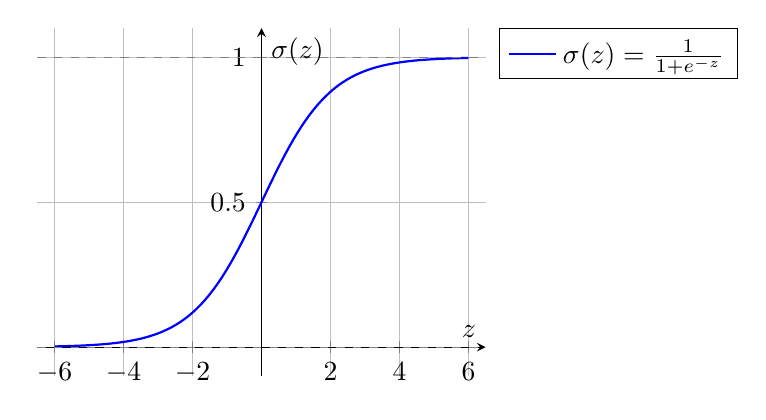
\begin{tikzpicture}
      \begin{axis}[
          width=0.6\textwidth, % Adjust width as needed
          height=6cm,
          axis lines=middle,
          xlabel={$z$},
          ylabel={$\sigma(z)$},
          grid=major,
          ymin=-0.1, ymax=1.1,
          xmin=-6.5, xmax=6.5,
          samples=100,
          domain=-6:6,
          legend pos=outer north east % Or other position
        ]
        \addplot [blue, thick] {1/(1+exp(-x))};
        \addlegendentry{$\sigma(z) = \frac{1}{1+e^{-z}}$}
        % Asymptotes
        \addplot [dashed, gray, domain=-6.5:6.5] {0};
        \addplot [dashed, gray, domain=-6.5:6.5] {1};
      \end{axis}
    \end{tikzpicture}
    \caption[Sigmoid Activation Function]{The Sigmoid activation function.}
    \label{fig:sigmoid_plot}
    \caption*{Own illustration.}
  \end{figure}


  \paragraph{Hyperbolic Tangent Function (\( \tanh \)):}
  The hyperbolic tangent function maps any real input to the range (-1, 1). It is defined as:
  \begin{equation}
    \tanh(z) = \frac{e^z - e^{-z}}{e^z + e^{-z}} = 2\sigma(2z) - 1
  \end{equation}
  It is frequently used as the main activation function for hidden states in RNNs and LSTMs (e.g., Equations~\ref{eq:rnn_hidden_state}, \ref{eq:lstm-candidate-cell}, \ref{eq:lstm-hidden-state}). See Figure~\ref{fig:tanh_plot}.

  \begin{figure}[htbp]
    \centering
    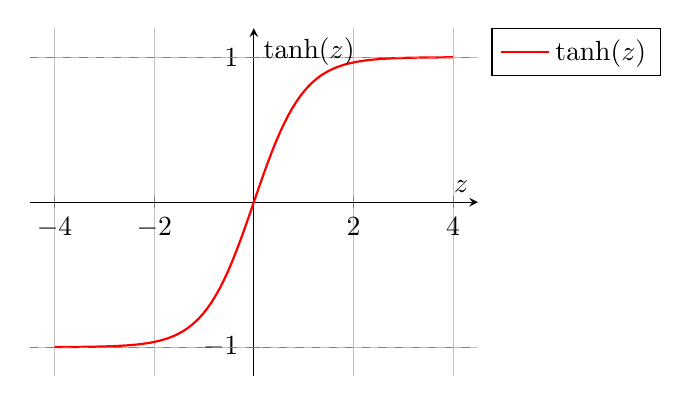
\begin{tikzpicture}
      \begin{axis}[
          width=0.6\textwidth,
          height=6cm,
          axis lines=middle,
          xlabel={$z$},
          ylabel={$\tanh(z)$},
          grid=major,
          ymin=-1.2, ymax=1.2,
          xmin=-4.5, xmax=4.5,
          samples=100,
          domain=-4:4,
          legend pos=outer north east
        ]
        \addplot [red, thick] {tanh(x)};
        \addlegendentry{$\tanh(z)$}
        % Asymptotes
        \addplot [dashed, gray, domain=-4.5:4.5] {-1};
        \addplot [dashed, gray, domain=-4.5:4.5] {1};
      \end{axis}
    \end{tikzpicture}
    \caption[Tanh activation function]{The Hyperbolic Tangent (tanh) activation function.}
    \label{fig:tanh_plot}
    \caption*{Own illustration.}
  \end{figure}


  \paragraph{Rectified Linear Unit (ReLU):}
  The ReLU function outputs the input directly if it is positive, and zero otherwise. It is defined as:
  \begin{equation}
    \text{ReLU}(z) = \max(0, z)
  \end{equation}
  ReLU is widely used in deep learning due to its simplicity and effectiveness in mitigating the vanishing gradient problem for positive inputs. It is used within the model presented in this thesis (Section~\ref{sec:integrated_architecture} refers to the code using it). See Figure~\ref{fig:relu_plot}.

  \begin{figure}[htbp]
    \centering
    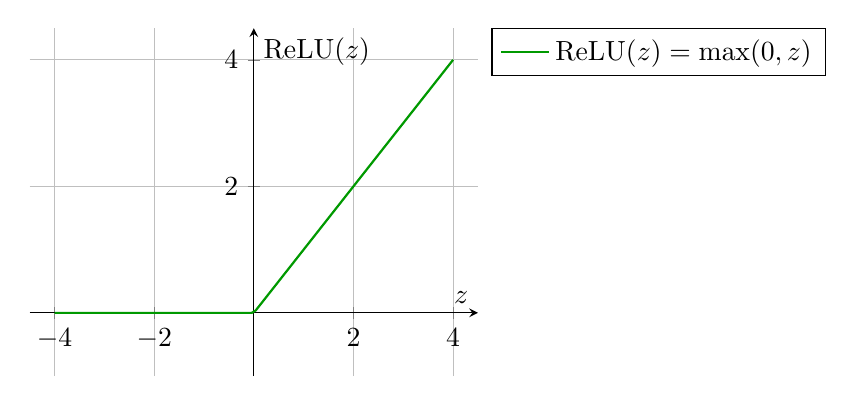
\begin{tikzpicture}
      \begin{axis}[
          width=0.6\textwidth,
          height=6cm,
          axis lines=middle,
          xlabel={$z$},
          ylabel={ReLU$(z)$},
          grid=major,
          ymin=-1, ymax=4.5,
          xmin=-4.5, xmax=4.5,
          samples=100,
          legend pos=outer north east
        ]
        \addplot [green!60!black, thick, domain=-4:4] {max(0,x)};
        \addlegendentry{ReLU$(z) = \max(0, z)$}
      \end{axis}
    \end{tikzpicture}
    \caption[ReLU activation function]{The Rectified Linear Unit (ReLU) activation function.}
    \label{fig:relu_plot}
    \caption*{Own illustration.}
  \end{figure}


  \paragraph{Softmax Function:}
  The softmax function converts a vector of K real numbers \( \bm{z} = (z_1, ..., z_K) \) into a probability distribution consisting of K probabilities. The function is applied to the entire vector and the \( i \)-th element of the output vector is calculated as:
  \begin{equation}
    \text{softmax}(\bm{z})_i = \frac{e^{z_i}}{\sum_{j=1}^K e^{z_j}} \quad \text{for } i = 1, ..., K
  \end{equation}
  The outputs are non-negative and sum to 1 (\( \sum_{i=1}^K \text{softmax}(\bm{z})_i = 1 \)). Softmax is commonly used in the output layer of multi-class classification models and plays a crucial role in normalizing scores into attention weights in the Attention mechanism (Equation~\ref{eq:scaled_dot_product_attention}).

  % -------------------------------------------------------------------------
  \subsection{Distance and Similarity Metrics}
  \label{subsec:distance_metrics}
  % -------------------------------------------------------------------------
  These metrics quantify the difference or similarity between vectors, which is fundamental in many machine learning tasks like clustering, nearest neighbour search, and evaluating embedding spaces. Let \( \bm{a}, \bm{b} \in \mathbb{R}^d \) be two vectors of dimension \( d \).

  \paragraph{Euclidean Distance (L2 Distance):}
  \label{eq:euclidean_distance}
  The most common distance measure, representing the straight-line distance between two points in Euclidean space. It is the L2 norm of the difference between the vectors:
  \begin{equation}
    d_{\text{Euclidean}}(\bm{a}, \bm{b}) = ||\bm{a} - \bm{b}||_2 = \sqrt{\sum_{i=1}^d (a_i - b_i)^2}
  \end{equation}

  \paragraph{Manhattan Distance (L1 Distance):}
  Measures the distance by summing the absolute differences of the vector components. It corresponds to the distance travelled along axes at right angles (like navigating city blocks). It is the L1 norm of the difference:
  \begin{equation}
    d_{\text{Manhattan}}(\bm{a}, \bm{b}) = ||\bm{a} - \bm{b}||_1 = \sum_{i=1}^d |a_i - b_i|
  \end{equation}

  \paragraph{Cosine Similarity:}
  Measures the cosine of the angle between two non-zero vectors, indicating their orientation similarity irrespective of their magnitude. It ranges from -1 (exactly opposite) through 0 (orthogonal) to 1 (exactly the same direction). It is calculated using the dot product and vector magnitudes (L2 norms):
  \begin{equation}
    \text{CosineSimilarity}(\bm{a}, \bm{b}) = \frac{\bm{a} \cdot \bm{b}}{||\bm{a}||_2 ||\bm{b}||_2} = \frac{\sum_{i=1}^d a_i b_i}{\sqrt{\sum_{i=1}^d a_i^2} \sqrt{\sum_{i=1}^d b_i^2}}
  \end{equation}
  Cosine similarity is widely used for comparing high-dimensional vectors, such as text document embeddings or feature vectors, where magnitude might be less important than orientation. Note that while similarity increases as the value approaches 1, Cosine Distance is sometimes defined as \( 1 - \text{CosineSimilarity}(\bm{a}, \bm{b}) \).

  % -------------------------------------------------------------------------
  \subsection{Attention Mechanism Components}
  % -------------------------------------------------------------------------
  % (Content from previous version - Dot Product, Scaling)
  The Scaled Dot-Product Attention mechanism (Equation~\ref{eq:scaled_dot_product_attention}) relies on several fundamental operations beyond the Softmax function:

  \paragraph{Dot Product Similarity:}
  The compatibility between a query \( \bm{q} \) and a key \( \bm{k} \) (both typically vectors of the same dimension \( d_k \)) is often computed using the dot product \( \bm{q} \cdot \bm{k} = \bm{q}^T \bm{k} \). As noted above, this is closely related to Cosine Similarity but does not normalize for vector magnitudes. For matrices \( Q \) and \( K \) containing multiple queries and keys as rows, the matrix product \( QK^T \) computes all pairwise dot products efficiently.

  \paragraph{Scaling:}
  To counteract the effect of large dot product values when the dimension \( d_k \) is high, the scores \( QK^T \) are scaled down by dividing by \( \sqrt{d_k} \) before applying the softmax function. This helps maintain a stable gradient flow during training.

  % -------------------------------------------------------------------------
  \subsection{Normalization Techniques}
  % -------------------------------------------------------------------------
  Normalization layers help stabilize training, speed up convergence, and sometimes improve generalization by standardizing layer inputs.

  \paragraph{Layer Normalization (LayerNorm):}
  Layer Normalization normalizes the inputs across the features for \textit{each individual data sample} in a batch, making its computation independent of the batch size. For an input vector \( \bm{x} \) representing the features for one sample at a specific layer, LayerNorm computes:
  \begin{equation}
    \text{LayerNorm}(\bm{x}) = \bm{\gamma} \odot \frac{\bm{x} - \mu_{\text{sample}}}{\sqrt{\sigma^2_{\text{sample}} + \epsilon}} + \bm{\beta}
    \label{eq:layernorm}
  \end{equation}
  Here, \( \mu_{\text{sample}} \) and \( \sigma^2_{\text{sample}} \) are the mean and variance calculated across the feature dimension(s) of the single input sample \( \bm{x} \). \( \bm{\gamma} \) (scale) and \( \bm{\beta} \) (shift) are learnable affine transformation parameters of the same dimension as \( \bm{x} \), and \( \epsilon \) is a small constant added for numerical stability. LayerNorm is frequently used in RNNs and Transformers (including the model implemented in this work) where batch statistics might be less stable or meaningful.

  \paragraph{Batch Normalization (BatchNorm):}
  (Included for contrast, delete if not relevant) Batch Normalization normalizes inputs across the \textit{batch dimension} for each feature separately. It calculates the mean \( \mu_{\text{batch}} \) and variance \( \sigma^2_{\text{batch}} \) for each feature across all samples in the current mini-batch. While highly effective in CNNs, its dependence on batch statistics can be less suitable for sequence models with variable lengths or small batch sizes compared to LayerNorm.

  % -------------------------------------------------------------------------
  \subsection{Pooling Strategies for Sequences}
  % -------------------------------------------------------------------------
  Pooling layers are used to aggregate information across the time or sequence dimension, often to produce a fixed-size representation from variable-length sequence outputs for downstream tasks like classification. Given a sequence of hidden states \( H = [\bm{h}_1, \bm{h}_2, ..., \bm{h}_T] \), where each \( \bm{h}_t \in \mathbb{R}^d \):

  \paragraph{Mean Pooling:}
  Calculates the element-wise average of the hidden state vectors across the sequence dimension:
  \begin{equation}
    \bm{h}_{\text{mean\_pool}} = \frac{1}{T} \sum_{t=1}^T \bm{h}_t
  \end{equation}
  The resulting vector \( \bm{h}_{\text{mean\_pool}} \in \mathbb{R}^d \) represents the average activation over the sequence. This strategy is used in the implemented model to summarize the output sequence before the final classification layer.

  \paragraph{Max Pooling:}
  Calculates the element-wise maximum of the hidden state vectors across the sequence dimension:
  \begin{equation}
    (\bm{h}_{\text{max\_pool}})_j = \max_{t=1...T} (\bm{h}_t)_j \quad \text{for } j = 1, ..., d
  \end{equation}
  The resulting vector \( \bm{h}_{\text{max\_pool}} \in \mathbb{R}^d \) captures the strongest activation for each feature dimension across the sequence.

  % -------------------------------------------------------------------------
  \subsection{Weight Initialization}
  % -------------------------------------------------------------------------
  Initializing the weight parameters of a neural network appropriately is crucial for effective training, helping to prevent issues like vanishing or exploding gradients.

  \paragraph{Kaiming (He) Initialization:}
  Proposed by He et al. \autocite{he2015delving}, this method is primarily designed for layers followed by Rectified Linear Unit (ReLU) activations. It accounts for the non-linearity of ReLU. For Kaiming Normal initialization (used in the implemented model via `kaiming_normal_`), weights \( W \) are drawn from a normal distribution \( \mathcal{N}(0, \text{std}^2) \), where:
  \begin{equation}
    \text{std} = \sqrt{\frac{2}{\text{fan\_in}}}
  \end{equation}
  Here, `fan_in` is the number of input units to the weight tensor. A variant considers the non-linearity slope \( a \) of leaky ReLU (where \( a=0 \) for standard ReLU).

  \paragraph{Xavier (Glorot) Initialization:}
  Proposed by Glorot and Bengio \autocite{glorot2010understanding}, this method aims to keep the variance of activations and gradients roughly constant across layers, particularly effective for symmetric activations like tanh or sigmoid. For Xavier Normal initialization, weights \( W \) are drawn from \( \mathcal{N}(0, \text{std}^2) \), where:
  \begin{equation}
    \text{std} = \sqrt{\frac{2}{\text{fan\_in} + \text{fan\_out}}}
  \end{equation}
  `fan_out` is the number of output units. Uniform versions also exist for both Kaiming and Xavier initialization.

  % -------------------------------------------------------------------------
  \subsection{Optimization Algorithms and Refinements}
  % -------------------------------------------------------------------------
  Optimization algorithms iteratively update model parameters \( \theta \) to minimize a loss function \( J(\theta) \).

  \paragraph{Stochastic Gradient Descent (SGD):}
  A fundamental algorithm that updates parameters based on the gradient of the loss computed on a small batch (or single sample) of data at iteration \( k \).
  \begin{equation}
    \theta_{k+1} = \theta_k - \eta \nabla J(\theta_k; \bm{x}^{(i)}; \bm{y}^{(i)})
  \end{equation}
  where \( \eta \) is the learning rate and \( \nabla J(...) \) is the gradient computed on a mini-batch \( (\bm{x}^{(i)}, \bm{y}^{(i)}) \). Variants include momentum or Nesterov momentum.

  \paragraph{Adam Optimizer:}
  \label{eq:adam}
  An adaptive learning rate optimization algorithm that computes individual adaptive learning rates for different parameters using estimates of first and second moments of the gradients \autocite{kingma2014adam}. It often converges faster than basic SGD. The update rules involve computing biased moment estimates (\( \bm{m}_t, \bm{v}_t \)), bias-corrected estimates (\( \hat{\bm{m}}_t, \hat{\bm{v}}_t \)), and then updating parameters:
  \begin{equation}
    \theta_{t+1} = \theta_t - \frac{\eta}{\sqrt{\hat{\bm{v}}_t} + \epsilon} \hat{\bm{m}}_t
    \label{eq:adam-update} % Reuse label if needed
  \end{equation}
  Adam is used for training the model in this work.

  \paragraph{Learning Rate Scheduling:}
  Techniques used to adjust the learning rate \( \eta \) during training, which can improve convergence and final model performance.
  \begin{itemize}
    \item \textit{ReduceLROnPlateau:} Monitors a specified metric (e.g., validation loss). If the metric does not improve for a defined number of 'patience' epochs, the learning rate is reduced by a multiplicative 'factor'. This strategy is employed in the training procedure of this thesis.
    \item \textit{Step Decay:} Reduces the learning rate by a fixed factor every specified number of epochs.
    \item \textit{Cosine Annealing:} Gradually decreases the learning rate following a cosine curve shape over a specified number of epochs or iterations.
  \end{itemize}

  % -------------------------------------------------------------------------
  \subsection{Loss Functions}
  % -------------------------------------------------------------------------
  % (Content from previous version - MSE, BCE, CCE - keep only relevant ones)
  Loss functions quantify the difference between the models predictions and the true target values, guiding the optimization process.

  \paragraph{Binary Cross-Entropy (BCE):}
  \label{eq:bce} % Reuse label if needed
  Used for binary classification tasks where the model outputs a probability \( \hat{p}_i \) for the positive class (true label \( y_i \in \{0, 1\} \)). It is the loss function used in the model training for this thesis.
  \begin{equation}
    \text{BCE} = -\frac{1}{N} \sum_{i=1}^N [ y_i \log(\hat{p}_i) + (1 - y_i) \log(1 - \hat{p}_i) ]
  \end{equation}

  % Remove MSE/CCE if not used elsewhere in the thesis

  % -------------------------------------------------------------------------
  \subsection{Regularization Techniques}
  % -------------------------------------------------------------------------
  % (Content from previous version - L2, Dropout)
  Regularization techniques are used to prevent overfitting by adding constraints or penalties to the model or its training process.

  \paragraph{L2 Regularization (Weight Decay):}
  Adds a penalty to the loss function proportional to the squared magnitude of the model weights \( \theta \).
  \begin{equation}
    J_{reg}(\theta) = J(\theta) + \frac{\lambda}{2} ||\theta||_2^2 = J(\theta) + \frac{\lambda}{2} \sum_i \theta_i^2
  \end{equation}
  where \( \lambda \) is the regularization strength. This encourages smaller weights.

  \paragraph{Dropout:}
  During training, randomly sets a fraction of neuron activations (outputs) to zero at each forward pass before the subsequent layer \autocite{srivastava2014dropout}. This prevents units from overly co-adapting and can be interpreted as training an ensemble of thinned networks. The dropout rate (e.g., 0.3 in the implemented model) specifies the probability of an element being zeroed out. At test time, dropout is turned off, and sometimes the outputs of the kept units are scaled down by the dropout rate (though often handled implicitly by libraries or absorbed into subsequent layers). Dropout is used in both the LSTM layers and the final fully connected block in the implemented model.

  % -------------------------------------------------------------------------
  \subsection{Data Handling for Sequences}
  % -------------------------------------------------------------------------

  \paragraph{Sequence Padding:}
  Neural networks typically require inputs within a batch to be tensors of uniform shape. Since sequential data (like manufacturing process steps or natural language sentences) often has varying lengths, techniques are needed to handle this during batch processing. Padding involves augmenting shorter sequences within a batch with special padding values (often zero) until they reach the length of the longest sequence in that batch. This results in rectangular tensors suitable for processing. The `collate\_fn` used in the data loading pipeline for this thesis employs padding (via `pad\_sequence`). It is important that subsequent computations (e.g., loss calculation, attention mechanisms) are designed to ignore or mask these padded values to avoid introducing noise.

  \chapter{Further Illustrations}

  \section{Design Science Research Methodology}
  \begin{figure}[H]
    \centering
    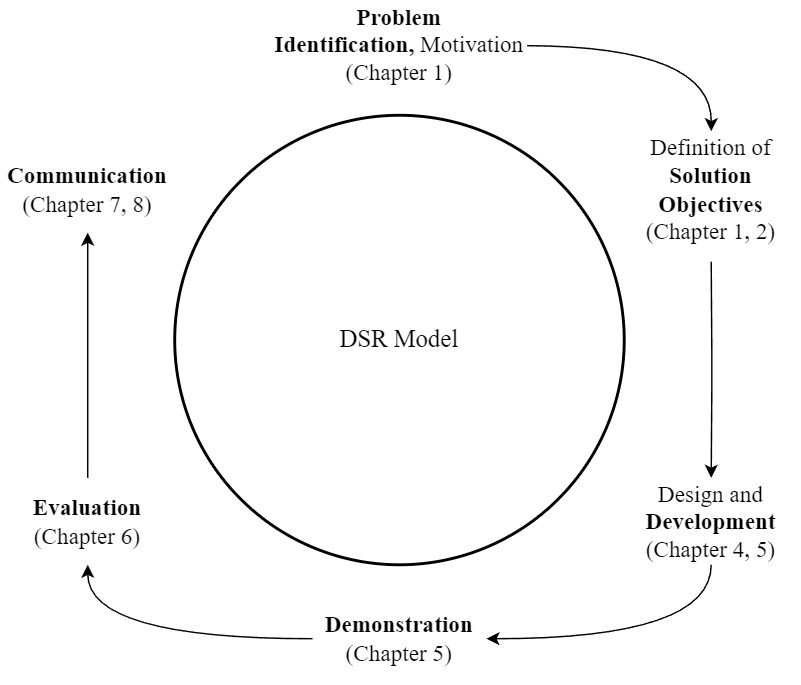
\includegraphics[width=0.6\textwidth]{figures/dsr.png}
    \caption[Design Science Methodology]{The cyclical design science research model. The model consists of six steps. The problem identification (1) refers to the research gap in automated VVUQ of SBDT. Defining the solution objectives (2) specifies the research gap by formulating questions and hypotheses based on the theoretical foundations. The design and development (3) phase includes the development of the framework. The demonstration (4) phase shows the application of the framework in a case study. The evaluation (5) phase assesses the effectiveness of the framework. The communication (6) phase concludes the research by presenting the results.}
    \label{fig:DSR}
    \caption*{Own illustration inspired by \textcite{peffers2007design}}
  \end{figure}

  \section{Time Encoding on Unit Circle}

  \begin{figure}[H]
    \centering
    \begin{tikzpicture}[
        scale=3, % Adjust scale to change overall size
        hour dot/.style={circle, fill=blue!70, inner sep=1.5pt},
        hour label/.style={font=\small}
      ]

      % Draw the unit circle
      \draw [gray, dashed] (0,0) circle (1);

      % Draw axes
      \draw [->, gray!80] (-1.3,0) -- (1.3,0) node[right, black] {$x_{\cos}$};
      \draw [->, gray!80] (0,-1.3) -- (0,1.3) node[above, black] {$x_{\sin}$};
      \node[above=5pt] at (current bounding box.north) {Hour of Day Encoded on Unit Circle}; % Title


      % Plot hour points and labels
      \foreach \h in {0,...,23} {
          % Calculate angle in degrees (TikZ trigonometric functions use degrees)
          \pgfmathsetmacro{\angle}{\h * 360 / 24}

          % Draw the point for the hour
          \node[hour dot] at (\angle:1) {}; % Place dot using polar coordinates (angle:radius)

          % Add labels for key hours slightly outside the circle
          \ifnum \h = 0 \node[hour label, anchor=west] at (\angle:1.15) {0h (Midnight)}; \fi
          \ifnum \h = 3 \node[hour label, anchor=south west] at (\angle:1.15) {3h}; \fi
          \ifnum \h = 6 \node[hour label, anchor=south] at (\angle:1.15) {6h (Morning)}; \fi
          \ifnum \h = 9 \node[hour label, anchor=south east] at (\angle:1.15) {9h}; \fi
          \ifnum \h = 12 \node[hour label, anchor=east] at (\angle:1.15) {12h (Noon)}; \fi
          \ifnum \h = 15 \node[hour label, anchor=north east] at (\angle:1.15) {15h}; \fi
          \ifnum \h = 18 \node[hour label, anchor=north] at (\angle:1.15) {18h (Evening)}; \fi
          \ifnum \h = 21 \node[hour label, anchor=north west] at (\angle:1.15) {21h}; \fi
        }

    \end{tikzpicture}
    \caption[Feature Transformation]{Sine and Cosine transformation of the hour of the day (0-23). Each hour is mapped to a point $(x_{\cos}, x_{\sin})$ on the unit circle (blue dots). Key hours are labelled, demonstrating how the transformation preserves cyclical continuity (hour 23 is near hour 0).}
    \label{fig:time-encoding}
    \caption*{Source: Own illustration}
  \end{figure}

  \chapter{Additional Statistical Validation Methods}
  \label{app:cct}

  This chapter details the methodology for the Cauchy Combination Test (CCT) and the Binomial test for rejection rates, which were used to provide a more robust statistical assessment of the significance observed across multiple runs of the permutation tests described in \autoref{sec:permtest}. These methods address the limitations of simply averaging p-values, particularly when dealing with potentially dependent results from repeated analyses on the same or related datasets.

  \section{Cauchy Combination Test (CCT)}
  \label{sec:cct_methodology}

  The Cauchy Combination Test \autocite{liu2020cauchy} provides a powerful method for combining $k$ individual p-values, $p_1, p_2, ..., p_k$, obtained from multiple statistical tests (in this case, the $k=10$ runs of the permutation test for each feature subset) into a single overall p-value. A key advantage of the CCT is its robustness under arbitrary dependence structures among the individual p-values, which is particularly relevant when tests are performed on resampled versions of the same underlying dataset.

  The CCT works by transforming each individual p-value $p_i$ using the inverse cumulative distribution function (CDF) of the standard Cauchy distribution ($C(0,1)$), which is equivalent to using the tangent function. Specifically, each $p_i$ is transformed into a Cauchy-distributed variable $t_i$:
  \begin{equation}
    t_i = \tan\left( (0.5 - p_i) \pi \right)
    \label{eq:cct_transform}
  \end{equation}
  where $\pi$ is the mathematical constant pi. Note that $p_i=0.5$ transforms to 0, $p_i \to 0$ transforms to $t_i \to \infty$, and $p_i \to 1$ transforms to $t_i \to -\infty$.

  The combined test statistic, $T_{CCT}$, is then calculated as the mean (or a weighted mean, though equal weights $w_i=1/k$ are typically used) of these transformed values:
  \begin{equation}
    T_{CCT} = \frac{1}{k} \sum_{i=1}^k t_i = \frac{1}{k} \sum_{i=1}^k \tan\left( (0.5 - p_i) \pi \right)
    \label{eq:cct_statistic}
  \end{equation}

  A remarkable property of the Cauchy distribution is that the average of $k$ independent standard Cauchy variables is itself a standard Cauchy variable. The CCT leverages the fact that this holds approximately even under dependence. Therefore, under the global null hypothesis (that all individual null hypotheses corresponding to $p_1, ..., p_k$ are true), the test statistic $T_{CCT}$ follows a standard Cauchy distribution, $C(0,1)$.

  The final combined p-value, $P_{CCT}$, is computed as the upper tail probability of the standard Cauchy distribution evaluated at the observed test statistic $T_{CCT}$:
  \begin{equation}
    P_{CCT} = P(C(0,1) \ge T_{CCT}) = 1 - F_{C(0,1)}(T_{CCT}) = 0.5 - \frac{\arctan(T_{CCT})}{\pi}
    \label{eq:cct_pvalue}
  \end{equation}
  where $F_{C(0,1)}$ is the CDF of the standard Cauchy distribution. A small $P_{CCT}$ indicates strong evidence against the global null hypothesis.

  The CCT is computationally simple and does not require estimating dependence structures. It is particularly powerful when the signal against the null hypothesis is sparse (i.e., present in only a subset of the individual tests) and maintains good performance under various dependency scenarios.

  \section{Binomial Test for Rejection Rate}
  \label{sec:binom_test_methodology}

  While the CCT combines the magnitude of the p-values themselves, the Binomial test provides a complementary perspective by formally assessing the significance of the observed \textit{Rejection Rate} ($RR$) \autocite{fahrmeir2016statistik}. The $RR$ is defined as the proportion of the $k$ individual runs for which the null hypothesis $H_0$ was rejected at a pre-defined significance level $\alpha$.
  This test addresses the question: "Is the number of times we rejected $H_0$ across the $k$ runs significantly greater than what we would expect purely by chance if $H_0$ were true for all runs?"

  Consider the $k$ runs of the permutation test performed for a specific feature subset. Let $\alpha$ be the significance level used for each individual run (e.g., $\alpha=0.05$ for DTree, $\alpha=0.01$ for BiLSTM). We define a "success" for a single run if its p-value $p_{run}$ is less than $\alpha$ ($p_{run} < \alpha$). Let $k_{obs}$ be the observed number of successful runs (i.e., number of rejections) out of the total $k$ runs. The Rejection Rate is $RR = k_{obs}/k$.

  The null hypothesis ($H_0$) for the Binomial test is that the true underlying probability of success (rejecting $H_0$ in any single run) is equal to the significance level $\alpha$. This assumes that under the global null, each run represents an independent Bernoulli trial with success probability $\alpha$.

  Under $H_0$, the random variable $X$ representing the number of successful runs follows a Binomial distribution with parameters $k$ (number of trials, i.e., runs) and $\alpha$ (probability of success):
  \begin{equation}
    X \sim B(k, \alpha)
  \end{equation}
  The probability of observing exactly $i$ successes in $k$ trials is given by the probability mass function (PMF) of the Binomial distribution:
  \begin{equation}
    P(X=i | k, \alpha) = \binom{k}{i} \alpha^i (1-\alpha)^{k-i}
    \label{eq:binom_pmf}
  \end{equation}
  where $\binom{k}{i} = \frac{k!}{i!(k-i)!}$ is the binomial coefficient.

  To assess whether the observed number of rejections $k_{obs}$ is significantly high, we compute the probability of observing $k_{obs}$ or more successes under $H_0$. This corresponds to a one-sided Binomial test p-value:
  \begin{equation}
    P_{Binom} = P(X \ge k_{obs} | H_0) = \sum_{i=k_{obs}}^{k} P(X=i | k, \alpha) = \sum_{i=k_{obs}}^{k} \binom{k}{i} \alpha^i (1-\alpha)^{k-i}
    \label{eq:binom_pvalue}
  \end{equation}
  A small $P_{Binom}$ suggests that observing $k_{obs}$ or more rejections is unlikely if the true rejection probability were only $\alpha$, providing evidence that the observed $RR$ is significantly higher than expected by chance and supporting the overall rejection of $H_0$ for that feature subset.

  This test directly quantifies the statistical significance of the consistency of rejecting $H_0$ across multiple independent or near-independent analyses, complementing methods like CCT that focus on the magnitude of the p-values.


  \section{Detailed Results for Decision Tree Model}
  \label{sec:dt_results_appendix}

  The following table presents the detailed hypothesis testing results obtained using the DTree as the model for distinguishing between real and simulated data. The evaluation metric was the ROC AUC score. The results are based on $k=10$ independent runs, each employing $N=1000$ permutations for p-value calculation. The significance level for individual run rejection and the Binomial test was set at $\alpha=0.05$. The Cauchy Combination Test (CCT) was used to combine p-values across runs (yielding $P_{CCT}$), and the Binomial test assessed the significance of the observed Rejection Rate ($RR$, yielding $P_{Binom}$).

  \begin{table}[htbp]
    \centering
    \caption[Detailed Decision Tree Model Results applying CCT]{Detailed Decision Tree validation results across 10 runs (N=1000, $\alpha=0.05$).}
    \label{tab:results-dt-appendix}
    \resizebox{\textwidth}{!}{%
      \begin{tabular}{l c c c c c p{3cm}}
        \toprule
        \textbf{Component ($\mathcal{F}_c$)} & \textbf{$\overline{\text{ROC AUC}}$} & \textbf{$\sigma_{\text{ROC AUC}}$} & \textbf{$P_{CCT}$} & \textbf{RR} & \textbf{$P_{Binom}$} & \textbf{Assessment} \\
        \midrule
        \texttt{time\_model}                 & 1.0000                               & 0.0000                             & 0.0000             & 1.00        & 0.0000               & INACCURATE          \\
        \texttt{resource\_model}             & 0.9817                               & 0.0088                             & 0.0000             & 1.00        & 0.0000               & INACCURATE          \\
        \texttt{transformation\_model}       & 1.0000                               & 0.0000                             & 0.0000             & 1.00        & 0.0000               & INACCURATE          \\
        \texttt{transition\_model}           & 1.0000                               & 0.0000                             & 0.0000             & 1.00        & 0.0000               & INACCURATE          \\
        \texttt{process\_model}              & 1.0000                               & 0.0000                             & 0.0000             & 1.00        & 0.0000               & INACCURATE          \\
        \texttt{kpi\_based}                  & 1.0000                               & 0.0000                             & 0.0000             & 1.00        & 0.0000               & INACCURATE          \\
        \texttt{all\_features}               & 1.0000                               & 0.0000                             & 0.0000             & 1.00        & 0.0000               & INACCURATE          \\
        \bottomrule
      \end{tabular}%
    }
    \caption*{Source: Own tabulation based on permutation test results.}
  \end{table}

  As evidenced by the results in Table \ref{tab:results-dt-appendix}, both the Cauchy Combination Test ($P_{CCT}=0.0000$) and the Binomial test ($P_{Binom}=0.0000$) yielded extremely significant p-values for all feature subsets when using the Decision Tree model at $\alpha=0.05$. The perfect rejection rate ($RR=1.00$) across all components further underscores this. This indicates a highly consistent and statistically robust ability of the DT model to distinguish between the real and simulated data across all evaluated components based on the engineered features, leading to the assessment "INACCURATE" for all components according to the defined validation framework.
  \section{Detailed Results for BiLSTM Model}
  \label{sec:lstm_results_appendix}

  The following table presents the detailed hypothesis testing results obtained using the BiLSTM classifier as the blackbox model for distinguishing between real and simulated data. The evaluation metric was the ROC AUC score. The results are based on $k=10$ independent runs, each employing $N=1000$ permutations for p-value calculation. The significance level for individual run rejection and the Binomial test was set at $\alpha=0.01$. The Cauchy Combination Test (CCT) was used to combine p-values across runs (yielding $P_{CCT}$), and the Binomial test assessed the significance of the observed Rejection Rate ($RR$, yielding $P_{Binom}$).

  \begin{table}[htbp] % Using htbp allows LaTeX more flexibility in placement
    \centering
    \caption[Detailed BiLSTM Model Results]{Detailed BiLSTM validation results across 10 runs (N=1000, $\alpha=0.01$).}
    \label{tab:results-lstm-appendix}
    \resizebox{\textwidth}{!}{%
      \begin{tabular}{l l l l l l p{3cm}}
        \toprule
        \textbf{Component ($\mathcal{F}_c$)} & \textbf{$\overline{\text{ROC AUC}}$} & \textbf{$\sigma_{\text{ROC AUC}}$} & \textbf{$P_{CCT}$} & \textbf{RR} & \textbf{$P_{Binom}$} & \textbf{Assessment} \\
        \midrule
        \texttt{time\_model}                 & 1.0000                               & 0.0000                             & 0.0000             & 1.00        & 0.0000               & INACCURATE          \\
        \texttt{resource\_model}             & 0.9945                               & 0.0071                             & 0.0000             & 1.00        & 0.0000               & INACCURATE          \\
        \texttt{transformation\_model}       & 1.0000                               & 0.0000                             & 0.0000             & 1.00        & 0.0000               & INACCURATE          \\
        \texttt{transition\_model}           & 0.9644                               & 0.1067                             & 0.0000             & 1.00        & 0.0000               & INACCURATE          \\
        \texttt{process\_model}              & 0.9714                               & 0.0858                             & 0.0000             & 1.00        & 0.0000               & INACCURATE          \\
        \texttt{kpi\_based}                  & 0.9975                               & 0.0054                             & 0.0000             & 1.00        & 0.0000               & INACCURATE          \\
        \texttt{all\_features}               & 1.0000                               & 0.0000                             & 0.0000             & 1.00        & 0.0000               & INACCURATE          \\
        \bottomrule
      \end{tabular}%
    }
    \caption*{Source: Own tabulation based on permutation test results.}
  \end{table}

  As shown in Table \ref{tab:results-lstm-appendix}, the results for the BiLSTM model are the same observed with the DTree. Using the stricter significance level of $\alpha=0.01$, both the CCT ($P_{CCT}=0.0000$) and the Binomial test ($P_{Binom}=0.0000$) yielded extremely significant p-values for all feature subsets. The rejection rate was also perfect ($RR=1.00$) across all components. This demonstrates a consistent and statistically robust capability of the BiLSTM model to distinguish between the real and simulated data across all SBDT components evaluated, leading to the assessment "INACCURATE" for all components within the validation framework.

\end{appendices}